% vim:textwidth=70
\chapter{分布式系统数据分发优化}
\label{chap:bt}

\section{本章引言}

%motivation: large file distribution in cooperative peers.
%problem: improve performance
% 说清楚一个应用场景,作为文章的backbone

数据分发技术是很多分布式应用的基础。P2P的文件共享系统将电影、歌曲和软
件CD等大文件分发给系统的每个用户。通过用户间合作下载,共享系统能够获得
几乎无限制的扩展性,同时,大大降低了数据源的负载。由文件共享系统产生的
数据传输,已经占了Internet流量的很大一部分。除此之外,人们还利用数据分
发技术,有效地将数据在CDN网络内部分发~\cite{fastreplica}。或者将这项技
术应用在分布式文件系统~\cite{sharkfs},让文件系统的用户安全地发现与下
载相互拥有的文件块,降低了服务器的压力。

数据分发的主要问题是将数据,尤其是大文件数据,分发到数量众多的用户或者
机器上。解决这个问题通常使用的基本技术是将文件分为逻辑上连续的若干块,
系统用户或者节点交换相互拥有的文件块,而不是直接向数据源服务器请求数据。
这样做的好处是显然的,首先降低了服务的压力,其次,这样的设计具有很好的
可扩展性,随着系统规模增大,总体的传输带宽也会增大。再次,文件块级别的
操作提供了更细粒度的负载均衡,从而系统节点能够动态的调整下载策略,绕开
可能的网络错误,以及获取更高下载性能。

进一步的,可以根据节点之间的通信拓扑将数据分发系统分为两种类型。swarm
类型的分发系统使用了随机连接拓扑,系统节点可以与任意其它节点通信。而
stream类型的系统使用了树、森林或者mesh等有约束结构的拓扑将节点连接起来。
swarm类型分发系统产生时间较stream类型系统更早。BitTorrent~\cite{bt}是
swarm系统的代表。BitTorrent使用一个集中式目录服务器记录系统节点与它们
下载文件的进度。BitTorrent的客户端之间通过这个目录服务器寻找可以提供文
件块下载其他节点。目前,一些基于BitTorrent协议的客户端也利用了
DHT~\cite{cademlia}技术,实现了分布式结构的目录服务器。基于stream方式
的分发系统,包括SplitStream~\cite{xxx}和Bullet~\cite{xxx}等,试图通过
使用精巧的节点选择算法来解决负载均衡和传输效率问题,其结果是使系统节点
构成了树、森林或mesh等结构拓扑,并且在分发过程中使这一结构尽量稳定。
这一方法带来的好处是可能获得更高的聚集带宽,然而这需要节点之间的行为很
好的同步,因而对底层网络提出了更高的要求。在节点之间不能很好同步的情况
下,stream类型系统的传输效率会降低。

一般来说,在Internet环境下基于swarm的分发技术得到了广泛应用。相比
stream类型系统,swarm更好的适应了Internet网络环境的动态变化,能够提供
良好的传输性能,同时也易于设计与实现。

% the point of paper
本文基于一个基本的问题:如何提高数据分发的性能?

% 通过比较相关工作,引出本文的内容
% 说明两种优化方法都是已有的,但是没有详细的研究

已有工作还有一些问题没有回答清楚。

% contribution?
通过广泛的模拟测试,我们得到了如下结论:

1. bns

2. bwalloc

3. lrf的影响

4. bns+bwalloc

再对结论小小的总结一下。

%\section{或者:临近节点选择、带宽分配、文件块选择}

\section{优化方法}

% 

\subsection{分发系统模型}

一般来说,一个数据分发系统可以用如下模型描述。

一个分发系统包括一个目录服务器和一组参与数据分发的节点。目录服务器维护
着节点列表与节点下载文件的进度。节点通过向目录服务器发送请求,获知系统
内其它节点的状态,包括节点列表与节点下载进度。同时,节点也会向目录服务
器更新自己的下载进度。分发系统的节点通过相互交换文件块完成文件下载,达
到数据分发的目的。

% 如何说的足够general,又能让基于bt的eval有说服力?

对一个分发系统来说,邻居选择、上传带宽分配和数据块选择是决定系统性能的
关键设计点。

邻居选择

% sharkfs: nearest peer, random piece, peer selection unspecified
% bittorrent: random peer, random/LRF, tit-for-tat
% 

% design figure

%节点选择和数据块选择的重要性。

本文考虑了两种提高分发性能的方法:选择临近节点作为邻居列表和动态上传带
宽分配。

\subsection{临近邻居选择}

%邻居选择,平均下载时间分析

临近邻居选择是指节点选择从“近”的邻居那里下载文件块。近的度量可以是节
点间延迟、带宽等网络连接属性,也可以是以延迟、带宽和丢包率为自变量的函
数值。从应用角度来看,以延迟时间(RTT)作为网络距离的度量是简单而有效
的方法。通常来看,延迟低的节点之间网络连接情况优于延迟高的节点。

% xxx: 分发树?and a bit of math

选择临近节点作为邻居列表从直观上来看是十分自然的。从单个节点来说,从近
处的节点下载文件块的速度更快,从而得到整个文件的时间更短。从整个分发系
统来说,完成整个文件分发的时间取决于每个文件块的分发时间,而每个文件块
的分发都动态构成一棵树。如果使用文件块传输时间为树上的边赋值,选择临近
节点后,分发树上的每条边的值以一定概率降低,从而整个分发性能得到提高。

临近节点选择方法,可以有两种实现方式。第一种

\subsection{上传带宽分配}

为了理解上传带宽分配方法,我们首先考虑一个简单的例子。考虑一个三个节点
构成的分发系统,$v_1$, $v_2$, $v_3$。$v_1$的上传带宽是1,而$v_2$和
$v_3$上传带宽是2,它们的下载带宽无限制。初始时刻,$v_1$上有大小为1的数
据块。$v_1$可以将上传带宽平均分给$v_2$和$v_3$,从而在时刻2,$v_2$和
$v_3$都得到了数据块,整个系统完成了数据分发。另外一种上传带宽分配是
$v_1$将带宽全部分给$v_2$,在时刻1,$v_2$得到了整个数据块,同时给$v_3$
上传数据。在1.5时刻$v_3$也得到了数据块。从而整个系统在1.5时刻就完成了
数据分发。如果系统中包含其它节点,在时刻1,$v_1$就可以向其它节点传输数
据,数据分发的效率更加提高。
% graph

上传带宽调度是怎么回事,

是贪心算法的应用

实现方式

\section{优化方法评测}

\subsection{评测方法}
模拟器, 128M
网络拓扑
节点加入退出
metrics
实验内容(bias,bwalloc,lrf...)

\subsection{biased neighbour}

% 现象、趋势、小结论、原因、前提条件,讨论配置变化的影响
% 每个subsection后给出一个总结
% 直接看图和表就能说明问题

我们首先测试了邻居节点选择对文件分发性能的影响。在测试中,节点每次向
tracker报告自己状态时,如果自身邻居节点数量少于设定值,会向tracker请求
返回系统内的若干随机节点(典型配置是50)最为自己的邻居。我们希望选择临
近的节点作为邻居会提高分发的性能,因而tracker返回的节点包括两部分:临
近节点和随机选择节点。但是这两部分节点的数量、比率在什么情况下会是最优
并不清楚。接下来我们试图通过实验测试的办法给出结论。

首先需要验证临近邻居节点选择是否会提升数据分发性能。我们设定临近比率是
80\%。也就是是在tracker返回的节点列表中,80\%是以网络延迟为距离定义,
离报告节点最近的一组节点,剩下20\%是从系统中随机选择的若干节点。这样做
的原因是避免由于全部邻居节点都按照最近距离选择,造成网络分割的现象。

\begin{figure}
  \centering
  \begin{minipage}{0.8\linewidth}
    \centering
    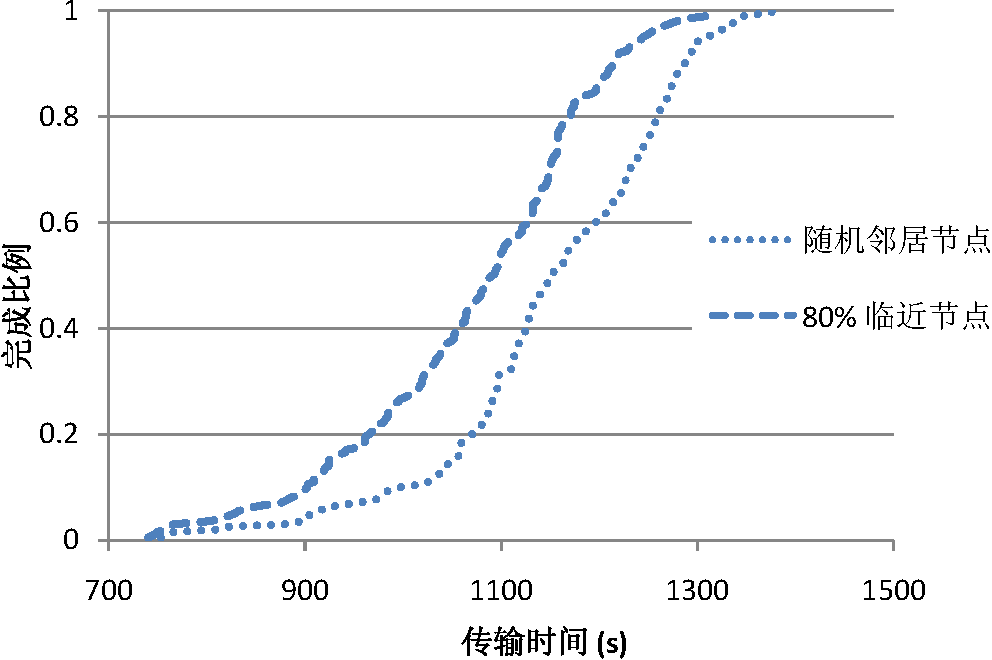
\includegraphics[width=1.0\linewidth]{bias80}
    \caption{临近邻居比率80\%时下载时间CDF曲线}
    \label{fig:bias80}
  \end{minipage}
\end{figure}

图~\ref{fig:bias80}是节点获取整个文件所用时间的累积分布函数(CDF),在
图中对比了使用随机邻居节点的结果和使用临近邻居节点选择后的结果。从
整体上来看,采用临近邻居节点选择后,曲线相比正常实现向左有明显移动。这
意味着相同数量的节点完成下载所需的时间更少了。为方便对比,图~
\ref{fig:bias80}上的关键统计数据总结在表~\ref{tbl:bias80}中。

可以看出,相比随机邻居选择,80\%比率的临近邻居选择对下载性能有了一定改
进。下载时间中值从1150秒下降到了1093秒,性能改进是5.0\%;90\%的节点完
成下载时间从1288秒下降到了1214秒,性能改进是5.7\%;下载时间的平均值从
1151秒下降到了1071秒,性能改进是7.0\%。

\begin{table}
\centering
\begin{minipage}{0.8\linewidth}
\centering
\caption{bias80}
\label{tbl:bias80}
\begin{tabular}{lccc}

\toprule[1.5pt]
    & 中值 & 90\%完成 & 平均值\\
\midrule[1pt]
随机邻居选择  & 1150s & 1288s & 1151s\\
80\% 临近邻居 & 1093s & 1214s & 1071s\\
性能改进      & 5.0\% & 5.7\% & 7.0\%\\
\bottomrule[1.5pt]
\end{tabular}
\end{minipage}
\end{table}

这样的结果是符合我们的预期的。然而相对来说,优化效果并不一定是最优的。
为了找到更优的邻居选择策略,我们变化临近邻居选择的比率,并观察对下载性
能的影响。图~\ref{fig:biaschange}是临近邻居比率从20\%变化到100\%时,下
载时间的平均值和中值的变化情况。

\begin{figure}
  \centering
  \begin{minipage}{0.8\linewidth}
    \centering
    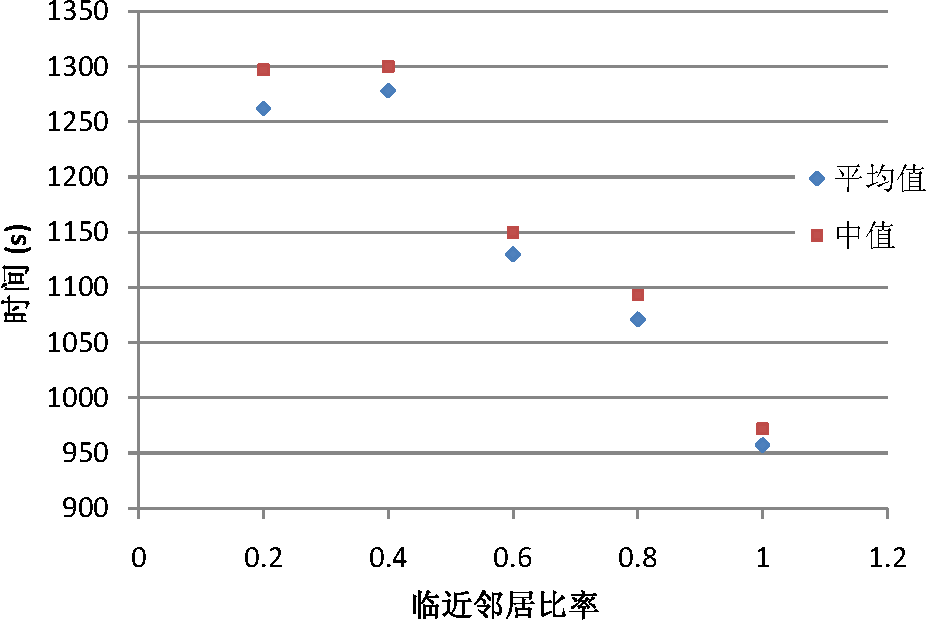
\includegraphics[width=1.0\linewidth]{biaschange}
    \caption{下载时间中值与平均值随临近邻居比率变化图}
    \label{fig:bias80}
  \end{minipage}
\end{figure}

可以看出,随着节点选择更多的临近邻居,系统的整体性能呈现单调增长的趋势。



在100\%


100\%也work

,因而提示我们xxx。

为了验证我们的想法,我们xxx。

图~\ref{fig:biask1}。

为了更仔细的研究系统特点,我们也收集了系统在分发文件过程中,节点的邻居
分布和系统总吞吐量的变化。
% path latency
% throughput

%1. 80\% bias: download time distribution, neighbour latency(需要重新测
%的), download rate from neighbours(可以从下载统计推导出)
%2. 不同bias
%3. 只保留若干长连接的bias

\subsection{带宽分配}
1. vs normal - download time (bwalloc)
2. 提高了整体throughput, (bwalloc\_throughput)
3. 与half,double对比 (bwalloc\_cmp)
4. 下载一个truck时间不好测,可以看从邻居下载速度是否增加,整体
throughput
5. 上传节点数量分布 (bwalloc\_upnode)
5. 原因:因为这个方法会选择上传的节点,和bias用latency选择类似。只不过
tracker没有帮助选择节点。比bias更好是因为分发truck的速度更快,考虑了自
身上传带宽的因素。

\subsection{lrf的影响}
1. 对bias的影响 (bias\_lrfvsrand)
2. 对带宽分配的影响 (bwalloc\_lrfvsrand)
3. diversity (almost ok, refine searchreast)
3. 原因: a) lrf会增进性能 b)对带宽分配优化影响相对小: bias以后,相近的
节点会有聚类效应,lrf能够很快的把类外的新的trunk拉回来。如果用random,
则很可能得到的trunk是类内的,分发数据的效率受影响。


\subsection{bias+带宽分配}
1. vs normal
2. 不具有叠加效果: xxx: bias以后,节点就已经比较近了,相互之间传输带宽
比较好,再使用带宽优化改进不大。

\section{实际应用的考量}
实现方式,优化效果

ISP的带宽分配、节流策略.

\section{相关工作对比}

1. 用bias优化bt:已有工作只是选择了一种bias方法使用,重点在如何实现
bias,例如用cdn,用landmark,但是我们系统评测了可能的bias方法,并给出
了最优结论:选择k=1

2. 带宽选择

3. lrf, seed对优化方法的影响

4. 两种优化方法不具有叠加效果。

5. 不同系统应用优化方法的建议

\section{结论}
